\item \textbf{{[}DHS/PRELIM/9597/2018/P1/Q4{]} }

Vector and matrix manipulation are used extensively in machine learning
programs. We will look at how common vector and matrix operations
are implemented using first principles 

\textbf{Addition and subtraction}

\texttt{{[}a,b,c{]} + {[}d,e,f{]} = {[}a+d,b+e,c+f{]}}

\texttt{{[}a,b,c{]} - {[}d,e,f{]} = {[}a-d,b-e,c-f{]}}

\textbf{Scalar multiplication} i.e. product of a constant and a vector 

\texttt{k {*} {[}a,b,c{]} = {[}k{*}a,k{*}b,k{*}c{]}}

\textbf{Dot product} (for 2 vectors of the same dimension)

\texttt{{[}a,b,c{]} $\cdot$ {[}d,e,f{]} = a{*}d + b{*}e + c{*}f}

\textbf{Distance} (between 2 vectors \texttt{{[}a,b,c{]}} and \texttt{{[}d,e,f{]}}
of the same dimension) 

$\sqrt{\left(\mathtt{a-d}\right)^{2}+\left(\mathtt{b-e}\right)^{2}+\left(\mathtt{c-f}\right)^{2}}$

\subsection*{Task 4.1 }

Using OOP techniques, create a class \texttt{Vector} to implement
the operations add, subtract, scalar multiplication, dot product and
distance. 

Exercise your class methods with the following vectors and constant: 

\texttt{v1 = {[}1,3,5{]}, v2 = {[}2,4,6{]}, k = 5}

\subsection*{Evidence 21 }

Program code. \hfill{}{[}12{]}

\subsection*{Evidence 22}

Screenshots. \hfill{}{[}2{]}

\subsection*{Task 4.2}

In some situations, it may be necessary to perform operations on vectors
of different dimensions eg for a convolution layer in deep learning.
The following diagram illustrates this process for a 3-element vector
\texttt{{[}1,2,3{]}} and a 5-element vector \texttt{{[}5,4,3,2,1{]}}.
The result will be a 3-element vector.
\begin{center}
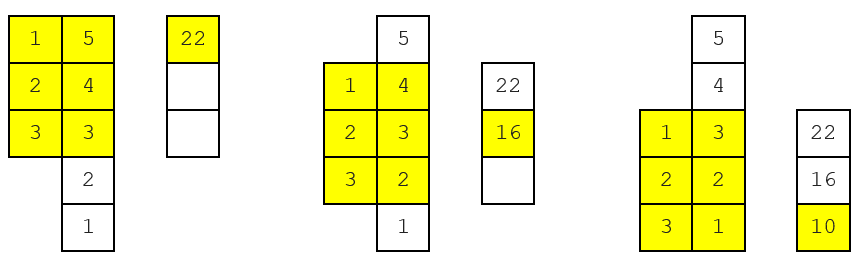
\includegraphics[width=0.5\paperwidth]{C:/Users/Admin/Desktop/Github/question_bank/LyX/static/img/9597-DHS-2018-P1-Q4-1}
\par\end{center}

Write program code to implement the convolution process for vectors.
Display the result to the screen.

\subsection*{Evidence 23 }

Program code. \hfill{}{[}5{]}

\subsection*{Evidence 24 }

Screenshot.\hfill{} {[}1{]}

\subsection*{Task 4.3 }

An example of the inner product for a matrix (2D array) is as follows:
\begin{center}
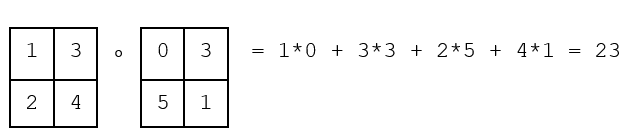
\includegraphics[width=0.5\paperwidth]{C:/Users/Admin/Desktop/Github/question_bank/LyX/static/img/9597-DHS-2018-P1-Q4-2}
\par\end{center}

Write program code to implement the convolution process for matrices
which uses the dot product for matrices. An example is shown below.
Display the result to the screen.
\begin{center}
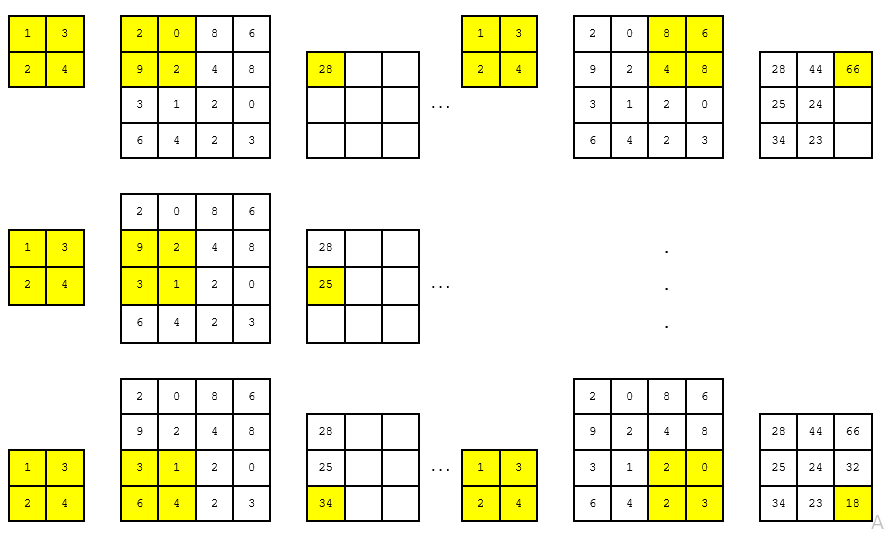
\includegraphics[width=0.65\paperwidth]{C:/Users/Admin/Desktop/Github/question_bank/LyX/static/img/9597-DHS-2018-P1-Q4-3}
\par\end{center}

\subsection*{Evidence 25 }

Program code. \hfill{}{[}8{]}

\subsection*{Evidence 26}

Screenshot.\hfill{} {[}2{]}